\chapter{Protótipo}

Este capítulo irá explorar os conceitos acerca do protótipo construído e detalhar como o mesmo foi montado e seu funcionamento.

\section{Objetivo do protótipo}
O protótipo foi desenvolvido pelo grupo com o objetivo de testar dois principais sistemas: controle e processamento de dados. O teste averiguará a eficiência dos códigos, bem como a resposta gerada pelas informações adicionadas na programação.
\section{Metodologia}
Para o protótipo foi montada uma lista de materiais, descritos mais adiante nesse relatório, e 4(quatro) reuniões para montagem do sistema. A parte de programação foi feita antes das reuniões, visto que o prazo para a entrega estava próximo. O valor dos materiais, bem como o transporte utilizado para a compra dos mesmos, foi divido com o grupo.
\section{Montagem}
Os materiais utilizados para a montagem (figura~\ref{fig1pr}) foram os seguintes:
\begin{itemize}
	\item   6 metros de mangueira para máquina de lavar;
	\item	4 válvulas mecânicas de 3cm de diâmetro;
	\item	8 conectores rosca/encaixe;
	\item	2 conectores tipo T de encaixe;
	\item	2 bombas para máquina de lavar; 
	\item	2 tubos de silicone pastoso;
	\item	2 coolers;
	\item	Placa Arduino;
	\item	Caixa de papelão;
	\item	Garrafa PET; 
	\item	Fita veda-rosca;
\end{itemize}
\begin{figure}[!htb]                  
	\centering                          
	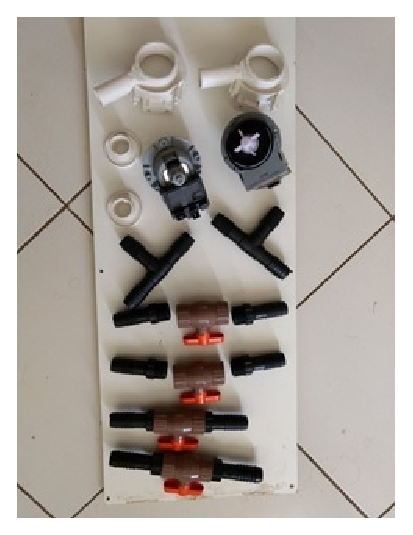
\includegraphics[scale=1]{figuras/figura1pr.eps}
	\caption{Conexões e bombas utilizadas} \label{fig1pr}              
\end{figure}	

Para a montagem do protótipo, o grupo mediu e cortou as mangueiras para o tamanho necessário e, em seguida, foram feitas e vedadas com silicone todas as conexões de encaixe, restando apenas as conexões de rosca. A bomba também necessitou de vedação, assim como as roscas, sendo estas vedadas com a fita \emph{veda-rosca}. A organização do sistema pode ser averiguada na figura ~\ref{fig1pr} , podendo-se destacar que o sistema não é cíclico neste protótipo. Visto que o propósito deste teste não era averiguar a capacidade do reservatório ou o funcionamento do sistema hidráulico, por isso o sistema manteve-se aberto, com água abastecendo a entrada e sendo coletada separadamente na saída.
\section{Funcionamento do Protótipo}
Para o primeiro teste, a água foi inserida na garrafa PET (representante do reservatório do sistema) com apenas duas das 4 válvulas abertas, uma bomba funcionando e um \textit{cooler} ligado. Nesse teste, o grupo buscou observar o comportamento do sistema quando dois dados fossem inseridos no código: aumento e diminuição de temperatura. Foi possível observar o sistema reagindo a esses dois comandos de modo que, no aumento da temperatura a bomba, funcionou de forma mais lenta e os \textit{coolers} de forma mais rápida. O inverso foi observado quando a temperatura diminuiu.\\
No segundo experimento, o grupo testou a eficiência do código de controle em requerer a troca das bombas. Foi adicionado ao código o dado do sensor de fluxo como nulo e, por consequência, pôde-se observar o desligamento de uma das bombas e o acionamento de outra.  
O terceiro teste consistiu em inserir um valor muito alto de temperatura e observar o acionamento da segunda bomba de água.\\
Com o protótipo pronto e testado (figura ~\ref{fig2pr}), o grupo conseguiu confirmar a eficiência dos códigos elaborados, bem como conferir a resposta dada por cada dado inserido neles.
\begin{figure}[!htb]                  
	\centering                          
	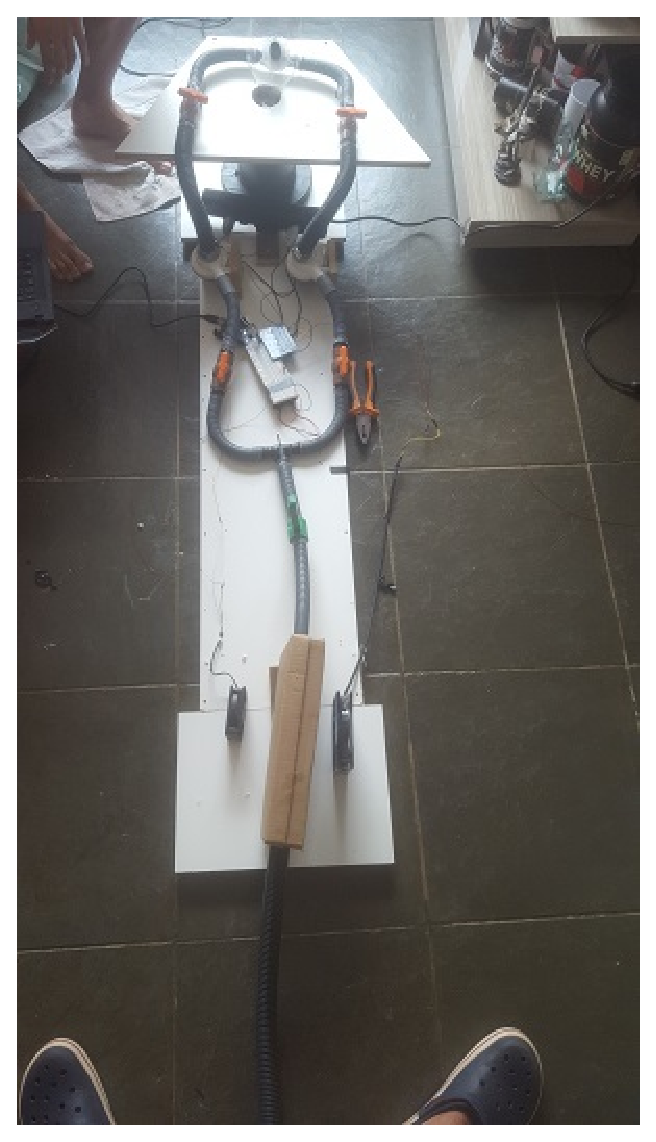
\includegraphics[scale=0.8]{figuras/figura2pr.eps}
	\caption{Protótipo construído} \label{fig2pr}              
\end{figure}
